\documentclass[a4paper,12pt]{article}

%% Language and font encodings
\usepackage[english]{babel}
\usepackage[utf8x]{inputenc}
%\usepackage[T1]{fontenc}

%% useful includes
\usepackage{amsmath}
\usepackage{amsfonts}
\usepackage{amssymb}
\usepackage{amsthm}
\usepackage{mathtools}

\usepackage[authoryear]{natbib}
\bibliographystyle{abbrv}

\usepackage{graphicx}
\usepackage{enumitem}
\usepackage{hyperref}


% %% Sets page size and margins
%\usepackage[a4paper,top=3cm,bottom=2cm,left=3cm,right=3cm,marginparwidth=1.75cm]{geometry}
\setlength{\parskip}{0.2em}




%% some useful commands

\renewcommand{\P}{\mathbf{P}}
\newcommand{\NP}{\mathbf{NP}}
\newcommand{\UP}{\mathbf{UP}}
\newcommand{\NPL}{\mathbf{NPL}}
\newcommand{\PLT}{\mathbf{PLT}}
\newcommand{\NPLMV}{\mathbf{NPLMV}}
\newcommand{\p}{\text{promise-}}
\newcommand{\co}{\text{co-}}
\renewcommand{\O}{\mathcal{O}}
\newcommand{\Lf}{\text{Leaf}}
\newcommand{\BL}{\text{BLeaf}}
\newcommand{\RLf}{\text{RLeaf}}
\newcommand{\RBL}{\text{RBLeaf}}
\newcommand{\ls}{\text{leafstring}}
\newcommand{\polylog}{\text{polylog}}
\newcommand{\faP}{\forall^{\text{P}}\cdot}
\newcommand{\exP}{\exists^{\text{P}}\cdot}
\newcommand{\faPL}{\forall^{\text{PL}}\cdot}
\newcommand{\exPL}{\exists^{\text{PL}}\cdot}

\newcommand{\In}{I n p u t: }
\newcommand{\Out}{O u t p u t: }
\newcommand{\Alg}{A l g o r i t h m: }



%% environments

\newtheorem{thm}{Theorem}[section]
\newtheorem{claim}[thm]{Claim}
\newtheorem{conj}[thm]{Conjecture}
\newtheorem{cor}[thm]{Corollary}
\newtheorem{definition}[thm]{Definition}
\newtheorem{lemma}[thm]{Lemma}
\newtheorem{problem}[thm]{Problem}

\theoremstyle{remark}
\newtheorem{remark}[thm]{Remark}
\newtheorem{example}[thm]{Example}
\newtheorem{examples}[thm]{Examples}

%\pagestyle{fancy}
%\fancyhead{}
%\fancyfoot{}
%\fancyhead[R]{\thepage}



\begin{document}

\section{A recursion formula for the coefficients}

\subsection{The coefficients of $\varrho_G$}

\begin{definition}
Let $A \in \mathbb{R}^{n \times n}$ symmetric, $v\in\mathbb{R}^n$. For arbitrary multiindices $I=(i_1, \ldots, i_k) \in \mathbb{N}^*$ with $0 \le i_1 < i_2 < \ldots < i_k$ define the coefficients $\delta_I$ by
\begin{align*}
\delta_i &\coloneqq \langle v, A^iv\rangle \text{ for $i \in \mathbb{N}$},\\
\delta_{(i_1, \ldots, i_k)} &\coloneqq \begin{cases*}
0 & if $i_j+1 = i_{j+1}$ for some $j$\\
\sum_{v\in\{0,1\}^{k-1}}(-1)^{|v|}\cdot\delta_{i_k-|v|}\cdot\delta_{(i_1,\ldots,i_{k-1})+v} & otherwise,
\end{cases*}
\end{align*}
where $|v| = \sum_{i=1}^kv_i$ denotes the number of ones in $v$.
\end{definition}

\begin{claim}
Let $A \in \mathbb{R}^{n \times n}$ symmetric, $v\in\mathbb{R}^n$, let $d \coloneqq \dim Z(v,A)$. For $i=0,\ldots,d$ define the vector $w^d_i\in\mathbb{N}^d$ by 
$$
w^d_i\coloneqq (0,2,4,\ldots, 2(i-1),2i+1,2(i+1)+1, \ldots, 2(d-1)+1).
$$
Then the characteristic polynomial of $A|_{Z(v,A)}$ is given by
$$
p(x) = \sum_{i=0}^d(-1)^{|w^d_i|} \cdot \frac{\delta_{w^d_i}}{\delta_{w^d_d}}x^i,
$$
where again $|w| \coloneqq \sum_{j=1}^k w_j$ denotes the $L^0$-norm of a vector.
\end{claim}

\begin{remark}
If $A$ satisfies $tr(A) \equiv 0 \mod 2$, then every $\delta_I$ for $I$ of length $k$ is divisible by $2^{k-1}$. If furthermore $n$ is even, every $\delta_I$ is divisible by $2^k$.
\end{remark}

\begin{remark}
For every $I$ of length $k > d$, it holds $\delta_I = 0$.
\end{remark}

\begin{proof}
It can be verified that the vectors
$$
v_j \coloneqq \sum_{l=0}^j (-1)^{|w^d_i|}\delta_{w^d_i}A^iv
$$
form an orthogonal basis of $Z(v,A)$. This implies, that the projection of $A^kv$ onto the subspace generated by $v, \ldots, A^{k-1}v$ has coordinates $(-1)^{|w^k_i|}\cdot \frac {\delta_{w^k_i}} {\delta_{w^k_k}}$ relative to the basis $v, \ldots, A^{k-1} v$. The assertion immediately follows.
\end{proof}

Hence, if $G$ is an undirected graph with adjacency matrix $A$, the above approach can be used to determine the recurrence polynomial $\varrho_G$.

\begin{remark}
A few comments on this approach:
\begin{enumerate}
\item Even when using dynamic programming, the recursion formula for the $\delta_I$ still has exponential complexity. 
\item The absolute value of the $\delta_I$ grows exponentially as well. Furthermore, in general the $\delta_I$ for multiindices of fixed length do not share a common factor other than $2^{k-1}$.
\item The most interesting question that arises: Why is every $\delta_{w_i^d}$ divisible by $\delta_{w_d^d}$? In particular, in general the coefficient $\delta_{w_d^d}$ seems to be a large square number. However, I could not prove this and there seem to be exceptions. Furthermore, I could not find any meaning of the square root of $\delta_{w_d^d}$.
\end{enumerate}
\end{remark}

\subsection{The recurrence degree of $G$}

If one is only interested in the recurrence degree of $G$, the following procedure describes a way to compute it in time $\mathcal{O}\left(n^3\right)$:

\begin{enumerate}[topsep=0pt,itemsep=-1ex,partopsep=1ex,parsep=1ex]
\item Initialize $B \coloneqq I_n, v \coloneqq (1, \ldots, 1), k \coloneqq n$
\item While $k>0$ do:
\item \quad $w \coloneqq v B$
\item \quad if $w = 0$:
\item \quad \quad return $n-k$
\item \quad pick $i\in\{1, \ldots, k\}$ with $w_i \neq 0$
\item \quad for $j \neq i$:
\item \quad \quad update the columns of $B\colon B_j \coloneqq w_i B_j - w_j B_i$
\item \quad delete the $i$-th column of $B$
\item \quad $v \coloneqq Av$
\item \quad $k \coloneqq k-1$
\item return $n$
\end{enumerate}

\section{Local recurrence polynomials}

\subsection{General theory}

There exists an isomorphism between the set of all linear recurrent sequences having characteristic polynomial $p$ and the quotient ring $\mathbb{Z}[x]/p(x)$ (see \cite{hall1938isomorphism}). If we identify the set of integer sequences with the ring of formal power series $\mathbb{Z}[[x]]$, this isomorphism is given by $\sigma(t) \mapsto p(t) t^{-1} \sigma\left(t^{-1}\right)$. The term $t^{-1}\cdot \sigma\left(t^{-1}\right) = \frac {r_\sigma(t)}{\varrho_\sigma(t)}$ (where $r$ and $\varrho_\sigma$ are coprime polynomials) is well-defined if and only if $\sigma$ is a linear recurrent sequence and $\varrho_\sigma(t)$ divides $p(t)$ if and only if $p$ is a characteristic polynomial for $\sigma$. In this case, $\varrho_\sigma$ is the least characteristic polynomial for $\sigma$.

Let $q(x)$ be the image of $\sigma \in \mathbb{Z}[[x]]$ in $\mathbb{Z}[x]/p(x)$. The sequence $\sigma$ has a characteristic polynomial $\varrho_\sigma$ of degree lower than $p$ if and only if $q(x) \in \mathbb{Z}[x]/p(x)$ is a zero divisor (if and only if $p$ and $q$ are not coprime). The polynomial $\varrho_\sigma$ is given by 
$$
\varrho_\sigma(x) = \frac {p(x)} {\gcd(p(x), q(x))}.
$$
Hence, if $q(x)$ is known, we can compute $\varrho_\sigma$ by factoring $p$ and $q$ (resp. in time $\mathcal{O}(n^2)$ with the Euclidean algorithm).

When the first $\deg(p)$ terms of $\sigma$ are known, it is possible to directly compute the polynomial $p(t) t^{-1} \sigma\left(t^{-1}\right)$. However, if $\sigma$ is the (local or global) walk count of a graph, this polynomial can be obtained in other ways.

\subsection{Undirected graphs}

Let $G$ be an undirected graph with adjacency matrix $A$ and let $u,v \in V$. The number of walks of length $k$ starting in $u$ and ending in $v$ is denoted by $w_k^{uv}$ and can be computed as $w_k^{uv} = \langle e_u,A^ke_v\rangle$. Denote the global walk count sequence of $G$ by $w_r$ and the images of $w_r$ resp. $w_r^{uv}$ in $\mathbb{Z}[x]/\chi_G[x]$ by $r_G$ resp. $r_{uv}$. By linearity of the described isomorphism it follows that $r_G = \sum_{u,v\in V}r_{uv}$. Hence, we are interested in computing the polynomials $r_{uv}$ for $u,v\in V$ arbitrary.

If $u=v$, this is relatively easy:

\begin{claim}\label{cl:closed_walks}
Let $G$ be an undirected graph with adjacency matrix $A$, $v\in V$. Then it holds
$$
r_{vv}(x) = \chi_{A_v}(x),
$$
where $A_v$ is obtained from $A$ by removing the $v$-th row and column.
\end{claim}

In other words, $r_{vv}$ is the characteristic polynomial of $G\backslash\{v\}$. In particular, it follows that $\varrho_{vv}$ consists of all factors of the characteristic polynomial of $A$ which are not contained in the characteristic polynomial of $A_v$. Furthermore, the previously described approach can be generalized to obtain that $\varrho_{vv}$ is the characteristic polynomial of $A|_{Z(e_v,A)}$.

If $u\neq v$, it gets more complicated. We say $p \in V^{k+1}$ is a simple path of length $k$, if $p = (v_1, \ldots, v_{k+1})$, such that the $v_i$ are pairwise unequal and $\{v_i,v_{i+1}\} \in E$ for all $i=1, \ldots, k$. In particular, the simple paths of length zero are exactly the nodes of $G$ and the simpe paths of length one are its edges (where each edge gives rise to two paths of length one). For nodes $u,v\in V$, let $P_{uv}$ be the set of simple paths starting in $u$ and ending in $v$.

\begin{claim}\label{cl:local_walks}
Let $G$ be an undirected graph with adjacency matrix $A$, let $u,v\in V$. Then it holds
$$
r_{uv}(x) = \sum_{p\in P_{uv}} \chi_{G\backslash p}(x).
$$
\end{claim}

Note, that this is a generalization of the previous Claim \ref{cl:closed_walks}. Using that $r_G = \sum_{u,v\in V}r_{uv}$, we get the following equation:
$$
r_G(x) = \sum_{p\subseteq G \text{ simple path}}\chi_{G\backslash p}(x).
$$
Therefore, the recurrence polynomial $\varrho_G$ consists of all factors of the characteristic polynomial, which do not divide this sum.

\begin{cor}
Let $d$ be the minimal degree among the degrees of the factors of the characteristic polynomial of $G$. If $G$ contains two nodes with (shortest path) distance $n-d$, then the characteristic polynomial of $G$ equals its minimal polynomial.
\end{cor}

Indeed, if $(u,v)$ is a pair of nodes with distance $n-d$, then the local residual $r_{uv}$ has degree $d-1$ (since the shortest path connecting $u$ and $v$ contains $n-d+1$ nodes) and can therefore not contain a factor of $\chi_G$. Hence, the local recurrence polynomial $\varrho_{uv}$ is equal to $\chi_G$. But since $\varrho_{uv}$ divides the minimal polynomial of $G$, they have to be equal.

\begin{figure}
\centering
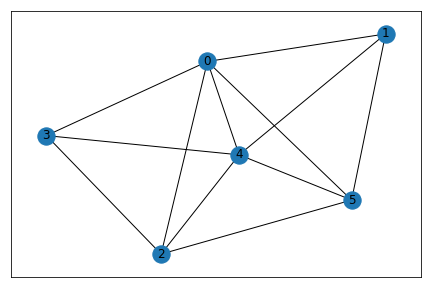
\includegraphics[scale=0.5]{pics/graph2.png}
\caption{Every local recurrence polynomial is a proper divisor of the minimal polynomial.}
\label{fig:proper_div}
\end{figure}

\begin{remark}
The local recurrence polynomials $\varrho_{uv}$ are always a factor of the minimal polynomial of $G$. However, $\varrho_{uv}$ can be a multiple of $\varrho_G$, a factor of $\varrho_G$ or neither of those. This can be seen for example in the path $P_4$ on five vertices. It holds
\begin{align*}
\varrho_G(x) &= x(x^2-3),\\
\varrho_{1,5}(x) &= x(x-1)(x+1)(x^2-3) = \chi_G,\\
\varrho_{1,3}(x) &= x(x^2-3),\\
\varrho_{2,3}(x) &= x^2-3,\\
\varrho_{2,4}(x) &= (x-1)(x+1)(x^2-3)
\end{align*}

In general however, we can make no statement about the local recurrence polynomials. There exist graphs where every local recurrence polynomial is a proper divisor of the minimal polynomial of $G$ (see Figure \ref{fig:proper_div}). On the other hand, there exist graphs where every local recurrence polynomial is equal to $\chi_G$, while $\varrho_G$ is a proper divisor of the characteristic polynomial (e.g. the path $P_3$).
\end{remark}


\begin{proof}
Proof of Claim \ref{cl:local_walks}.

\noindent Rough idea: First use that $\varrho_{uu}$ is equal to the characteristic polynomial of $A$ restricted to $Z(e_u,A)$, to show the claim for closed walks.

Afterwards: Every walk from $u$ to $v$ can (uniquely) be decomposed as $(v_0=u, C_0, v_1, C_1, \ldots,v_{n-1}, C_{n-1}, v_n=v, C_n)$, where $(u, v_1, \ldots, v_{n-1}, v)$ is a simple path and every $C_i$ is a closed walk on $v_i$ not passing through any $v_j$ for $j < i$. This should lead to the desired result.
\end{proof}

\begin{cor}
Let $G$ be an undirected graph, $u \in V$, let $d \coloneqq \max_{v\in V}(\text{dist}(u,v))$. Then the local recurrence polynomial $\varrho_{uu}$ has degree at least $d+1$.
\end{cor}

\begin{proof}
Recall that $\varrho_{uu}$ is te characteristic polynomial of $A|_{Z(e_u,A)}$. Since $\left(A^ie_u\right)_v = 0$ for all $i < d$, but $\left(A^de_u\right)_v > 0$, the vector $A^de_u$ is linearly independent of all $A^ie_u$ for all $i < d$. Hence, $\deg\left(\varrho_{uu}\right) = \dim\left(Z(e_u,A)\right) \ge d+1$.
\end{proof}

\begin{cor}
Let $G$ be an undirected graph, $u,v\in V$. Then $\varrho_{uv}$ is a divisor of $\varrho_{uu}$.
\end{cor}

\begin{proof}
Let $\varrho_{uu} = x^d - \sum_{i=0}^{d-1} \beta_ix^i$. Then it holds that
$$
A^ke_u = \sum_{i=k-d}^{k-1}\beta_iA^ie_u
$$
for all $k \ge d$. In particular, this implies
$$
w_k^{uv} = \langle e_u, A^de_v\rangle = \sum_{i=k-d}^{k-1}\beta_i\langle e_u, A^ie_v\rangle = \sum_{i=k-d}^{k-1}\beta_iw_i^{uv}
$$
and hence, $\varrho_{uu}$ is a characteristic polynomial for $w_r^{uv}$ as desired.
\end{proof}

Unfortunately, in general $\varrho_{uv}$ is a proper divisor of the greatest common divisor of $\varrho_{uu}$ and $\varrho_{vv}$.

\bibliography{references.bib}
\end{document}
